\chapter{Regresión Cuantil y Datos Funcionales}\label{RegCuanDatosFun}

En esta sección se presentarán conceptos esenciales para el desarrollo matemático fundamental de la investigación. Se comenzará abordando conceptos básicos de probabilidad y el modelo de regresión cuantil, acompañados de ejemplos clásicos para una comprensión más profunda de su funcionamiento.


%%%%%%%%%%%%%%%%%%%%%%%%%%%%%%%%%%%%%%%%%%%%%%%%%
%%%%%% CONCEPTOS ESENCIALES DE PROBABILIDAD %%%%%
%%%%%%%%%%%%%%%%%%%%%%%%%%%%%%%%%%%%%%%%%%%%%%%%%

\section{Conceptos Esenciales}

A toda variable aleatoria (v.a.) se le asocia una función de distribución, la cual es de vital importancia porque contiene toda la información relevante sobre la variable aleatoria y la medida de probabilidad asociada a sus posibles valores. Se representa como el total de masa acumulada a la izquierda hasta en punto $x$ incluyendo este. A continuación, se presenta su definición \cite{Rincon}.

\begin{defn}[Función de Distribución]
    La función de distribución de una variable aleatoria $X$ es la función $F: \mathbb{R} \to [0, 1]$, definida como sigue

    \begin{equation}\label{distF}
        F(x) = \mathbb{P}(X \leq x).
    \end{equation}
\end{defn}

La función definida en \eqref{distF}, es monótona no decreciente, continua por la derecha, con límite por la izquierda y, $F(-\infty) = 0$ y $F(\infty) = 1$. Este concepto se puede extender a un vector de variables aleatorias, lo que resulta en una función multivariada como a continuación se menciona. 

\begin{defn}[Función de Distribución Conjunta]
    La función de distribución de un vector $X = (X_1, \dots , X_n)$ denotada por $F: \mathbb{R}^{n} \to [0, 1]$, se define como sigue:

    \begin{equation}
        F(x_1, x_2, \dots, x_n) = \mathbb{P}\left ( X_1 \leq x_1, X_2 \leq x_2, \dots, X_n \leq x_n \right ).
    \end{equation}
\end{defn}

En situaciones prácticas, típicamente se dispone de una muestra fija del vector aleatorio, donde estas observaciones representan las variables predictoras. En muchos casos, no se cuenta con información detallada sobre la distribución marginal de cada variable o la distribución conjunta. Por lo tanto, para inferir sobre estas distribuciones, se aplican técnicas de estimación. La distribución empírica de una variable aleatoria se define de la siguiente manera:

\begin{defn}[Distribución Empírica]
 Dada una muestra $(x_1, x_2, \dots, x_n)$, donde cada $x_i$ es una observación proveniente de la v.a. $X$ y es independiente de las otras observaciones, la función de distribución empírica se define como:

\begin{equation}\label{fdaEmp}
    \widehat{F}(x)=\frac{1}{n} \#\left\{i \in\{1,2, \ldots, n\}: x_i \leq x\right\}=\frac{1}{n} \sum_{i=1}^n \mathbf{1}\left(x_i \leq x\right), \quad x \in \mathbb{R},
\end{equation}    
\end{defn}

$\widehat{F}$ es un estimador de la función de distribución $F$ de un conjunto de datos dado.

Por otro lado, la función cuantil corresponde a la función inversa generalizada de la función de distribución. Representa una herramienta esencial en estadística y probabilidad. Esta función proporciona una manera de relacionar valores específicos de una distribución de probabilidad y los percentiles correspondientes. Es decir, dada una probabilidad o percentil determinado, la función cuantil devuelve el valor en el que la distribución alcanza o supera esa probabilidad. A continuación, se proporciona la definición.

\begin{defn}\label{defcuantil}
    A cualquier función de distribución $F$ se le asocia la función cuantil $Q$, definida por:
    
    \begin{equation}\label{eqdefcuantil}
        Q(p) = \inf \left\{ x \in \mathbb{R}: F(x) \geq p \right\}, \quad p \in [0, 1],
    \end{equation}
    
    donde $\inf$ representa el ínfimo con la convención de $\inf \emptyset = \infty$ \cite{CopulasR}.
    \end{defn}

%falta cunatil empiric
La función cuantil empírica proporciona una forma de estimar cuantiles a partir de los datos observados, sin hacer suposiciones sobre la forma específica de la distribución subyacente. En lugar de utilizar una fórmula analítica, la función cuantil empírica ordena los datos observados y selecciona el valor correspondiente a la posición fraccionaria que representa el cuantil deseado.


\begin{defn}[Función Cuantil Empírica]
    Dada una muestra $x_1, x_2, \dots, x_n$, donde cada $x_i$ es una observación proveniente de la v.a. $X$ y es independiente de las otras observaciones y, $x_{(1)}, \dots, x_{(n)}$ los estadísticos de orden asociados. La función cuantil empírica se define como:

    \begin{equation}
        \widehat{Q}(u) =  \inf \left\{ x: \frac{1}{n}\sum _{i = 1}^{n}  1(x_{(i)} \leq x) \geq u\right\}. 
    \end{equation}
\end{defn}

Más adelante, al modelar variables utilizando cópulas, se asumirá que cada distribución marginal es una variable aleatoria uniforme estándar. Por lo tanto, en seguida, se presenta la transformación integral de probabilidad o \textit{Probability Integral Transform} (PIT), la cual establece una relación entre la función de distribución de una variable aleatoria y una variable aleatoria uniforme estándar. Esta transformación es fundamental para entender cómo las distribuciones de diferentes variables se relacionan entre sí y cómo se pueden utilizar variables uniformes estándar para simular y modelar distribuciones más complejas en el contexto de cópulas \cite{CopulasR}.

\begin{defn}[Transformación integral de probabilidad]\label{PITdef}
    Si $X \sim F$ es una variable aleatoria continua y $x$ es un valor observado de $X$, entonces la transformación $u := F(x)$ se denomina transformación integral de probabilidad (PIT) en $x$.
\end{defn}

\begin{obs}\label{PITdist}
    Si $X \sim F$, entonces $U := F(X)$ está distribuida de forma uniforme. Primero nótese que $U \in [0, 1]$ y además, 

    \begin{equation}
        P(U \leq u)=P(F(X) \leq u)=P\left(X \leq F^{-1}(u)\right)=F\left(F^{-1}(u)\right)=u,
    \end{equation}

    la cual es función de distribución de la uniforme estándar.
\end{obs}


%%%%%%%%%%%%%%%%%%%%%%%%%%%%%%%%%%%%%%%%%%%%%%%%%
%%%%%%%%%%%%%% REGRESION CUANTIL %%%%%%%%%%%%%%%%
%%%%%%%%%%%%%%%%%%%%%%%%%%%%%%%%%%%%%%%%%%%%%%%%%

\section{Regresión Cuantil}
    
    La regresión cuantil es una técnica estadística utilizada para modelar la relación entre la variable predictora y una variable respuesta, centrándose en diferentes cuantiles de la distribución condicional de la variable de respuesta, comúnmente la mediana \cite{cuantilReg}. Esta técnica fue introducida por Koenker y Bassett en 1978.  
    
    A diferencia de la regresión clásica por mínimos cuadrados que se centra en estimar la media condicional de la variable de respuesta, la regresión cuantil se centra en cómo varía la relación entre las variables a lo largo de diferentes cuantiles de la distribución condicional. Esta tiene dos principales ventajas sobre la regresión lineal:
    
    \begin{enumerate}
        \item No hace ningún supuesto sobre la distribución de la distribución de la variable respuesta.
        \item Esta es más robusta ante la presencia de datos atípicos. 
    \end{enumerate}

    Un cuantil especifico puede ser encontrado resolviendo el siguiente problema de Teoría de Decisiones. Sea $\rho_\tau(u)$ la función de pérdida dada en la ecuación \eqref{funPer}, la cual es equivalente a las expresiones que se muestran en la ecuación \eqref{alternativas}. En la Figura \ref{fig:perdida} se muestra la gráfica de la función $\rho_\tau(u)$.
    
    \begin{equation}\label{funPer}
    \rho_\tau(u)= u\left(\tau-\mathbb{I}_{(u<0)}\right)
    \end{equation}

    \begin{equation}\label{alternativas}
    \begin{split}
        &\rho_\tau(u)=\max \{(\tau-1) u, \tau u\}\\
        &\rho_\tau(u)=\left(\tau-\frac{1}{2}\right) u+\frac{1}{2}|u|
    \end{split}
    \end{equation}
    
    \begin{figure}[H]
        \centering
        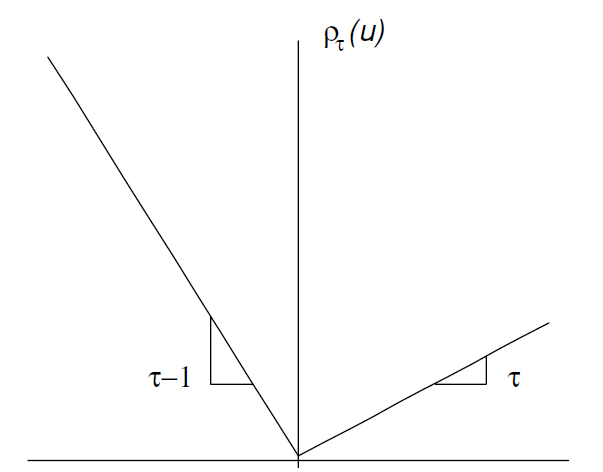
\includegraphics[width = 0.5 \textwidth]{Imagenes/perdida.png}
        \caption{Función de pérdida.}
        \label{fig:perdida}
    \end{figure}
    
    El $\tau$-ésimo cuantil se puede calcular al minimizar la función de pérdida evaluada en $X-u$ con respecto a $u$ como se muestra a continuación \cite{Koenker2005}
    
    \begin{equation}\label{minCun}
        Q_X(\tau)=\underset{u}{\arg \min } E\left(\rho_\tau(X-u)\right)=\underset{u}{\arg \min }\left\{(\tau-1) \int_{-\infty}^u(y-u) d F(x)+\tau \int_u^{\infty}(x-u) d F(x)\right\} .
    \end{equation}

    Esto se puede ver si se calcula la derivada de la ecuación \eqref{minCun} con respecto a $u$ y se igual a $0$

    \begin{equation}\label{perdidaF}
        0=(1-\tau) \int_{-\infty}^{u} d F(x)-\tau \int_{u}^{\infty} d F(x)=F(u)-\tau.
    \end{equation}

    Para el caso empírico la fórmula queda de la siguiente manera, 

    \begin{equation}\label{qestima}
        \widehat{Q}_{X}(\tau)=\arg \min _{u_\tau \in \Re}\left\{\sum_{X_i \geq u_\tau} \tau \left(X_i-u_\tau\right)+\sum_{X_i< u_\tau}(1-\tau) \left(u_\tau-X_i\right)\right\}.
    \end{equation}

    Así para un conjunto de covariables $X$, es posible ajustar una regresión $\widehat{Q}$ parra el $\tau$-ésimo cuantil de una variable respuesta usando la función de pérdida \eqref{qestima}.

    Existe varios métodos más generales de estimación de modelos de funciones cuantiles condicionales como mínimos cuadrados. Minímos cuadrados proporciona una proporciona una forma relativamente sencilla de obtener los parámetros. Para el caso donde $T = 0.5$ y los distribución de los errores son normales, se tiene la regresión lineal clásica \cite{Koenker2005}. En la Figura \ref{fig:regQ}\footnote{Figura tomada de \cite{ImgRegCuantile}}, se muestra un ejemplo de este ajuste a diferentes niveles de percentiles.

    \begin{figure}[H]
    \centering
    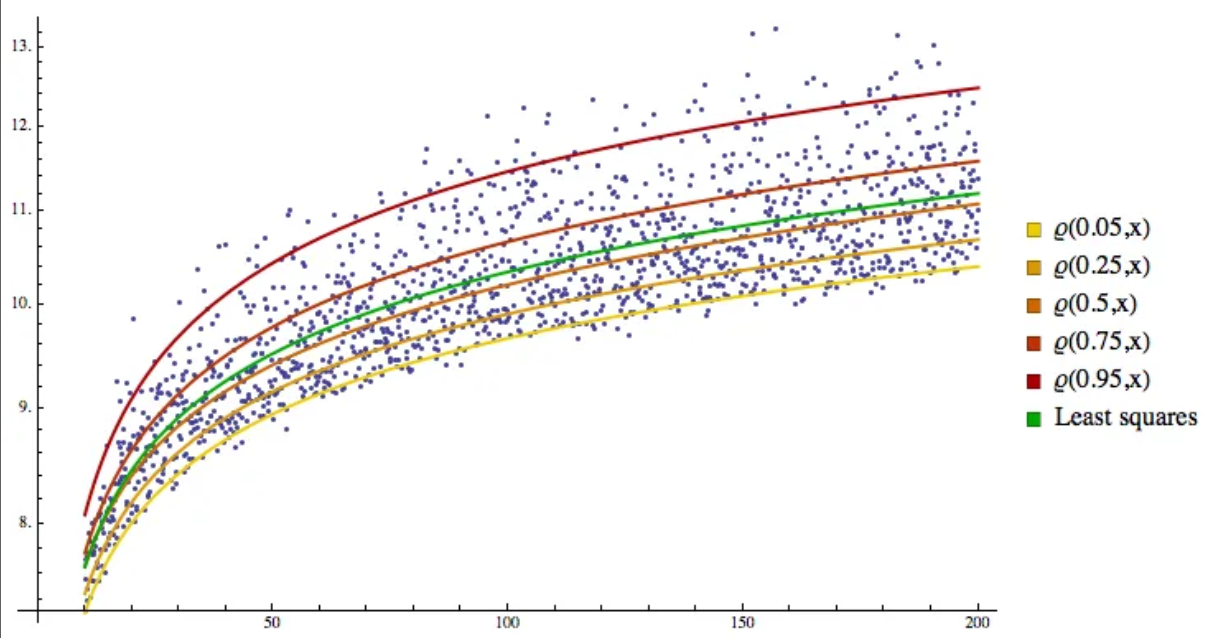
\includegraphics[width = 0.9 \textwidth]{Imagenes/Quantilsregression.png}
    \caption{Ejemplo del ajuste empleando la regresión cuantil a diferentes niveles de percentiles.}
    \label{fig:regQ}
    \end{figure}
    
%%%%%%%%%%%%%%%%%%%%%%%%%%%%%%%%%%%%%%%%%%%%%%%%%%%%%
%%%%%%%%%% Ejemplo con regresión lineal %%%%%%%%%%%%%
%%%%%%%%%%%%%%%%%%%%%%%%%%%%%%%%%%%%%%%%%%%%%%%%%%%%%

\begin{obs}[Regresión Cuantil Lineal]
    Como se hace en la clásica regresión lineal, se define $Y_i=\beta_{0, \tau}+\beta_{1, \tau} \cdot X_i+\varepsilon_{i, \tau} \quad \forall i \in\{1, \dots n\}$ con $0 < \tau < 1$, donde $\tau$ corresponde al $\tau$-ésimo cuantil de error con respecto a la variable respuesta, es decir, $Q(\varepsilon_{i, \tau}) = 0$. Entonces, usando la fórmula \eqref{qestima} se obtiene la siguiente ecuación

    \begin{equation}
        \hat{\beta}_\tau=\arg \min _{\beta_\tau \in \mathbf{R}^2}\left\{\sum_{Y_i \geq A} \tau \left|Y_i-\beta_{0, \tau}-\beta_{1, \tau} X_i\right|+\sum_{Y_i<A}(1-\tau) \left|Y_i-\beta_{0, \tau}-\beta_{1, \tau}  X_i\right|\right\}
    \end{equation}

    donde $\beta_\tau = (\beta_{0, \tau}, \beta_{1, \tau} )$ y A = $\beta_{0, \tau} + \beta_{1, \tau}X_i $. Por lo que, resolver la estimación de parámetros se convierte en un problema de programación lineal \cite{RegLinealCuantil}.
\end{obs}

%%%%%%%%%%%%%%%%%%%%%%%%%%%%%%%%%%%%%%%%%%%%%%%%%%%%%%%%%%%%%
%%%%%%%%%%  D A T O S  F U N C I O N A L E S  %%%%%%%%%%%%%%%
%%%%%%%%%%%%%%%%%%%%%%%%%%%%%%%%%%%%%%%%%%%%%%%%%%%%%%%%%%%%%

\section{Datos Funcionales}

Los datos funcionales son una forma de representar información que varía de manera continua en una dimensión o más dimensiones, como el tiempo, el espacio u otras variables continuas. En muchos experimentos estadísticos, las observaciones son funciones por naturaleza, como curvas temporales o superficies espaciales, donde la unidad básica de información es la observación funcional. Esto contrasta con los datos tradicionales, que suelen consistir en observaciones puntuales o discretas.

Un ejemplo ilustrativo de las ventajas de usar datos funcionales, tomado de \cite[Pág. 6]{Ramsay2009}, se encuentra en un estudio realizado en el hospital de San Diego. Este estudio se centró en medir el ángulo formado entre la cadera y la rodilla durante el ciclo de caminada. A diferencia de otros enfoques que se basaban en datos discretos, este estudio empleó datos funcionales para modelar la continuidad del movimiento, proporcionando una representación más detallada y precisa del ángulo a lo largo del ciclo completo. En la Figura \ref{ejemplo1}\footnote{Figura tomada de \cite{Ramsay2009}} se ilustra los datos funcionales. El intervalo $[0,1]$ representa un ciclo único y las curvas punteadas muestran la extensión periódica de los datos más allá de cualquiera de los extremos del ciclo. La ventaja de modelarlo como un continuo radica en la capacidad de capturar con mayor precisión las variaciones sutiles y los patrones dinámicos del ángulo a lo largo del ciclo completo, considerando los estados anteriores y proporcionando una representación más detallada y realista del movimiento.

\begin{figure}[H]
 \centering
  \subfloat[Ángulo formado entre la cadera y la rodilla]{
   \label{ejemplo1}
    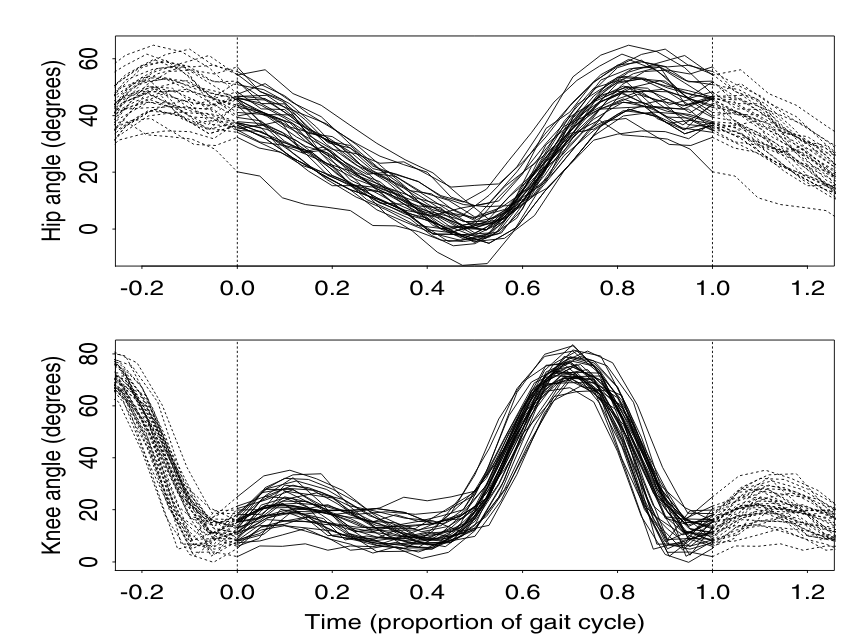
\includegraphics[width=0.45\textwidth]{Imagenes/functionalDataEj1.png}}
  \subfloat[Manuscritos]{
   \label{ejemplo2}
    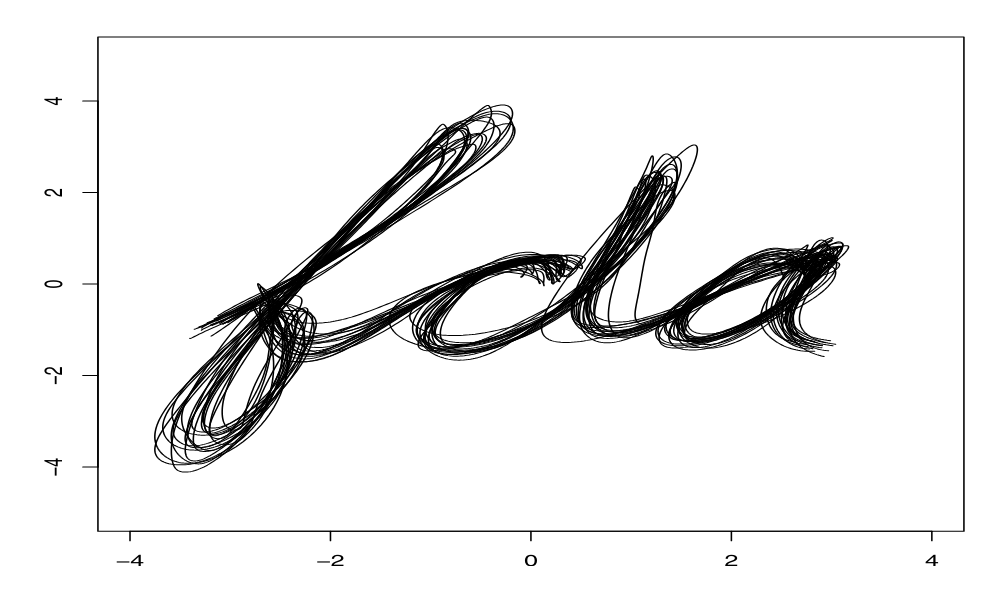
\includegraphics[width=0.45\textwidth]{Imagenes/functionalDataEj2.png}}
    \caption{Ejemplos de datos funcionales.}
    \label{fig:fdaEjemplo}
\end{figure}

Como se mencionó anteriormente, una de las utilidades de los datos funcionales es modelar el movimiento. Un caso de esta aplicación se muestra en la Figura \ref{ejemplo2} \footnote{Figura tomada de \cite{Ramsay2009}}, donde se presentan $20$ superposiciones de manuscritos. Este enfoque permite capturar las modificaciones tenues y los patrones inherentes en cada trazado, proporcionando una representación más precisa y detallada de los movimientos involucrados en la escritura \cite[Pág. 8]{Ramsay2009}.

Los datos funcionales permiten capturar la evolución de una variable a lo largo de una dimensión continua. Se emplean en una amplia gama de campos, incluyendo la estadística, la econometría, la neurociencia, la meteorología y muchas otras áreas donde es esencial modelar y comprender la evolución continua de los fenómenos \cite{boxplotFun}.

\subsection{Representación de Datos}

No siempre es posible realizar mediciones de los experimentos de interés como un continuo debido a diversos factores, como la complejidad de la medición. Por esta razón, a menudo se dispone de una serie de datos discretos que representan estas funciones. Para superar esta limitación, se utilizan técnicas de regresión y smoothing. La regresión permiten crear una función continua que ajusta los datos discretos, mientras que el smoothing ayuda a reducir el ruido y las irregularidades en los datos, proporcionando una representación más suave y precisa del movimiento.

Los datos funcionales típicamente consisten en una muestra aleatoria $x_1(t), \dots , x_n(t)$ de funciones independientes de variable real de un proceso estocástico $X(t)$ tal que $X(t) \in \mathbb{R}$,  donde $t \in \mathcal{T}$ y $\mathcal{T}$ es un intervalo en $\mathbb{R}$. Los datos funcionales se representan en enrejados discretos y finitos y comúnmente contienen errores de medición. Esto significa que, en lugar de tratar con funciones continuas en un dominio infinito, se trabaja con un conjunto finito de puntos de datos que se distribuyen a lo largo del dominio de interés. Cada punto de datos representa el valor de la función en un momento específico. Un modelo típico para las observaciones es:

\begin{equation}
     X_i(t_{il}) = \widetilde{X}_i(t_{il}) + \epsilon_{il},
\end{equation}

donde $X_i(t_{il})$ es el valor observable en $t_{il} \in \mathcal{T}$, $l = 1, \dots, L_{i}$, $i = 1, \dots, n$, $\widetilde{X}_i(t)$ es la función subyacente (suave) y $\epsilon_{il}$ son los términos de ruidos los cuales son independientes e idénticamente distribuidos \cite{Gertheiss}.

Como parte del análisis, es de interés reconstruir la función subyacente $\widetilde{X}$. Como paso inicial, se realiza un suavizamiento de la curva, tratándolo como un problema de regresión no paramétrica \cite{Gertheiss}. Entre los métodos más utilizados para este propósito se encuentran: 

\begin{itemize}
    \item Kernel Smoothing: Este método suaviza la curva utilizando un promedio ponderado de los datos cercanos, donde los pesos disminuyen con la distancia.

    \item Local Polynomial Smoothing: Similar al suavizamiento por kernel, este método ajusta un polinomio a los datos dentro de una ventana móvil. 

    \item Spline or Penalized Spline Approaches: Estos métodos utilizan funciones spline, que son piezas de polinomios ajustadas a intervalos del dominio de los datos. Los splines penalizados incluyen un término de penalización para evitar sobreajustes.
\end{itemize}

Para ejemplificar esto, se expandirá $\widetilde{X}_i = \widetilde{X}_i(\cdot)$ en una base splines. Se asume que este puede ser aproximado como una combinación lineal de splines base denotados como $\phi_{k}$, $k = 1, \dots, K$. Entonces,

\begin{equation}
     X_i(t_{il}) = \widetilde{X}_i(t_i{il}) + \epsilon_{il} = \sum_{k = 1}^{K}\phi_k(t_{il})\theta_{ik} + \epsilon_{il}
\end{equation}

con coeficientes desconocidos $\theta_{ik}$ que son estimados usando alguna técnica de optimización. 

\begin{figure}[H]
    \centering
    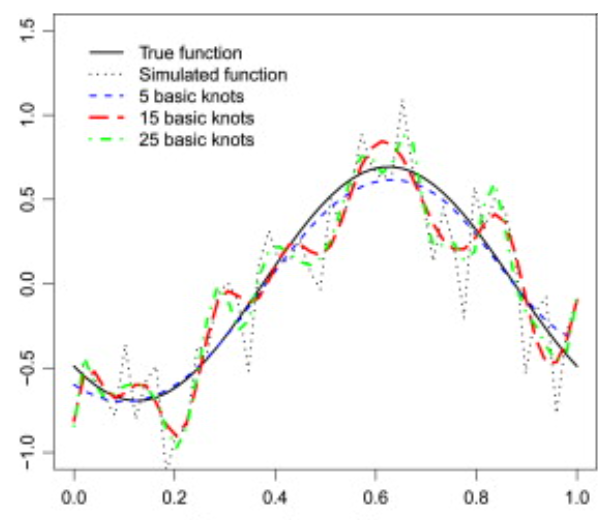
\includegraphics[width = 0.6\textwidth ]{Imagenes/splineEj.png}
    \caption{Aproximación usando splines.}
    \label{fig:ejSpline}
\end{figure}


En la Figura \ref{fig:ejSpline} \footnote{Figura tomada de \cite{Aguilera2013}}, se muestra un ejemplo de aproximación utilizando splines. Esta muestra la aproximación a la función subyacente, marcada en negro, usando datos con ruido (línea punteada) y diferentes números de splines. Un mayor número de splines produce un peor ajuste a la función subyacente, ya que no filtra el ruido de manera eficiente. Lo cual presenta un nuevo reto: determinar el número óptimo de splines para aproximar mejor la función. Por ejemplo, se ha abordado este problema utilizando splines adaptativos, validación cruzada, métodos de penalización entre otros \cite{Aguilera2013}.


Los datos funcionales continuos pueden ser complejos y difíciles de manejar debido a su naturaleza infinita. Al discretizar los datos en puntos finitos, se simplifican los cálculos y se facilitan las operaciones computacionales. Las discretizaciones permiten aplicar técnicas estadísticas y métodos de análisis de datos estándar  \cite{Aguilera2013}.

%%%%%%%%%%%%%%%%%%%%%%%%%%%%%%%%%%%%%%%%%%%%%%%%%%%%%%%%%%
\subsection{High Frequency}

En muchos campos científicos, los datos se recopilan a escalas de tiempo cada vez más finas, resultando en lo que se conoce como datos de alta frecuencia o \textit{High Frequency}. Estos datos capturan eventos y cambios con una resolución temporal muy detallada, permitiendo un análisis más granular y preciso de los fenómenos estudiados. Un ejemplo de la aplicación de este tipo de datos es en finanzas, donde la alta frecuencia permite comprender mejor las microestructuras del mercado \cite{Tsay2000}.

 En aplicaciones como el análisis de movimiento humano o la escritura a mano, los datos funcionales derivados de datos de alta frecuencia ofrecen una representación más realista y detallada, permitiendo una comprensión más profunda de los fenómenos estudiados. Los datos funcionales son especialmente aplicables con datos de alta frecuencia porque las herramientas estadísticas de FDA suelen depender de alguna forma de suavizado para transformar datos de alta dimensión o incompletos en una curva más suave. Esta curva puede ser descrita por un número menor de parámetros o un modelo parámetro, facilitando así el análisis y la interpretación de datos complejos y detallados \cite{Miao2013}.

 
%%%%%%%%%%%%%%%%%%%%%%%%%%%%%%%%%%%%%%%%%%%%%%%%%%%%%%%%%%

\subsection{Banda de Profundidad para Datos Funcionales}

Una de las grandes dificultades al realizar el análisis de datos funcionales es poder establecer comparaciones sobre la distribución de estos datos. Sin embargo, esta tarea se complica aún más cuando se trata de datos funcionales multivariados. A diferencia de los datos tradicionales, donde la escala es la principal herramienta de comparación, en el caso de los datos funcionales, lo relevante es su forma a lo largo del tiempo o de otra dimensión continua.

Por esta razón, López-Pintado y Romo introdujeron una noción de bandas de profundidad, la cual permite asignarles un orden teniendo en cuenta los aspectos anteriormente mencionados, es decir, una noción de estadísticos de orden con datos funcionales \cite{RomoPintado}. Estas bandas de profundidad proporcionan una forma de comparar y ordenar datos funcionales multivariados, lo que facilita su análisis y comprensión en estudios estadísticos y científicos. Posteriormente, Ying Sun y Marc Genton desarrollaron una metodología para crear boxplots con datos funcionales en su artículo `Functional Boxplots' \cite{boxplotFun}.

Sea $x_{[i]}(t)$ la curva muestral asociada al $i$-ésimo dato más profundo. Se denotará por $x_{[1]}(t), \dots, x_{[n]}(t)$ a los estadísticos de orden, donde $x_{[1]}(t)$ representa la curva más profunda y central, o la mediana, mientras que $x_{[n]}(t)$ representa la curva más atípica.


\begin{defn}[Banda]
    Se define la gráfica de la función $x(t)$ como un subconjunto en el plano $G(x) =  \left\{ (t, x(t)): t \in \mathcal{I} \right\}$. Se define la banda delimitada por las curvas $x_1, \dots, x_n$ como,
    
    \begin{equation}
        B\left(x_{i_1}, \ldots, x_{i_k}\right)=\left\{(t, u(t)): t \in \mathcal{I}, \min_{r=1, \ldots, k} x_{i_r}(t) \leq u(t) \leq \max _{r=1, \ldots, k} x_{i_r}(t)\right\}.
    \end{equation}
\end{defn}

\begin{defn}[Banda de Profundidad Poblacional]
    Sea $J$ el número de curvas que determinan la banda, donde $J$ es número fijo entre $2 \leq J \leq n$. Para copias $x_1(t), \dots, x_n(t)$ independientes de un proceso $X(t)$, la banda de profundidad poblacional definida para una curva $x(t)$ con respecto a la medida de probabilidad $P$, se define como:

    \begin{equation}
        \mathrm{BD}_J(x, P)=\sum_{j=2}^J \mathrm{BD}^{(j)}(x, P)=\sum_{j=2}^J P\left\{G(x) \subset B\left(X_1, \ldots, X_j\right)\right\},
    \end{equation}

    donde $B(X_1, \dots, X_j)$ es la banda delimitada por $j$ curvas aleatorias.
\end{defn}

La versión muestral de la $\mathrm{BD}^{j}(x, P)$ es obtenida calculando la fracción de bandas determinadas por $j$ diferentes observaciones que contienen la gráfica de $x(t)$

\begin{equation}
    \mathrm{BD}_n^{(j)}(x)= \binom{n}{j}^{-1} \sum_{1 \leq i_1<i_2<\cdots<i_j \leq n} \mathbbm{1}\left\{G(x) \subseteq B\left(x_{i_1}, \ldots, x_{i_j}\right)\right\}.
\end{equation}

En otras palabras, se está calculando la proporción de bandas que contiene a la de gráfica $x(t)$. Esto implica que cuanto mayor sea esta fracción, más central será la posición de la curva. En términos prácticos, una fracción más grande indica que la curva es más cercana a la gráfica `central'.

Así, la profundidad muestral de banda de la gráfica $x(t)$ está determinada por

\begin{equation}
    \mathrm{BD}_{n, J(x)} = \sum_{j = 2}^{J} \mathrm{BD}_n^{(j)}(x).
\end{equation}

Para comprender mejor cómo calcular la profundidad de banda, a continuación se presenta un ejemplo sencillo que involucra cuatro observaciones, el cuál es tomado de \textit{Functional Boxplots} \cite{boxplotFun}.

\begin{ejemplo}
   En la Figura \ref{fig:CurvasX}\footnote{
Figura tomada de \cite{boxplotFun}}, se muestra un escenario con 4 observaciones. Para calcular la profundidad de cada observación, es necesario construir las bandas considerando grupos de $2, 3$ y $4$ observaciones.
    
    Para $J = 2$ hay $6$ posibles bandas, es decir las combinaciones de $4$ en $2$, las cuales son $B(x_1, x_2)$, $B(x_1, x_3)$, $B(x_1, x_4)$, $B(x_2, x_3)$, $B(x_2, x_4)$ y $B(x_3, x_4)$. En la Figura \ref{fig:CurvasX}, se muestra en gris la banda entre $x_1$ y $x_3$, y se puede apreciar que las curvas que contiene esta banda son $x_1, x_2$ y $x_3$. En la Ecuación \eqref{j2}, se muestran todas las bandas con las curvas que contienen cada una.
    
    \begin{equation}\label{j2}
        \begin{matrix}
        x_1,x_2 \subseteq  B(x_1, x_2),  & x_2,x_3 \subseteq  B(x_2, x_3), \\
        x_1,x_2, x_3 \subseteq  B(x_1, x_3),  & x_2,x_4 \subseteq  B(x_2, x_4), \\
        x_1,x_2, x_4 \subseteq  B(x_1, x_4),  & x_3,x_4 \subseteq  B(x_3, x_4), \\
    \end{matrix}
    \end{equation}

    Por lo tanto, la profundidad de banda muestral para $j = 2$ de cada observación es la siguiente:

    \begin{equation}
        \begin{matrix}
            \mathrm{BD}^{2}_4(x_1) = \frac{3}{6}, & \mathrm{BD}^{2}_4(x_2) = \frac{5}{6},  & \mathrm{BD}^{2}_4(x_3) = \frac{3}{6},  & \mathrm{BD}^{2}_4(x_4) = \frac{3}{6}. \\
        \end{matrix}        
    \end{equation}
    
    \begin{figure}[H]
    \centering
    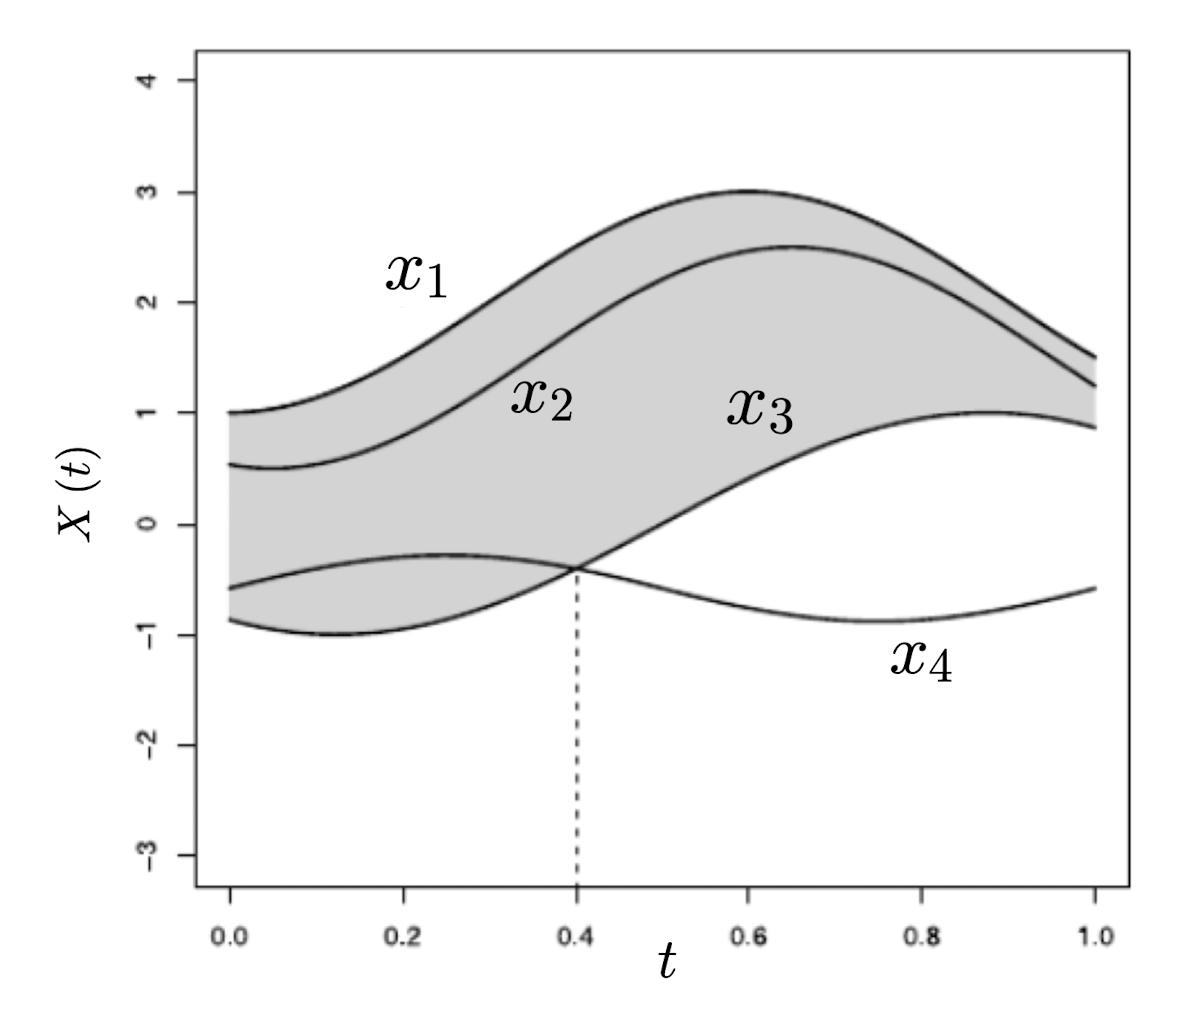
\includegraphics[width = 0.6 \textwidth]{Imagenes/WhatsApp Image 2024-04-21 at 8.06.25 PM.jpeg}
    \caption{Ejemplo de gráfico para la medida de profundidad.}
    \label{fig:CurvasX}
\end{figure}

Ahora, hay que repetir el proceso para $J = 3$. En la Ecuación \eqref{j3} se muestran las bandas y sus respectivas observaciones que están contenidas. En la Ecuación \eqref{BDJ3} se muestra el nivel de profundidad de cada observación.

\begin{equation}\label{j3}
    \begin{matrix}
        x_1, x_2, x_3 \subseteq B(x_1, x_2, x_3), & x_1, x_2 x_3, x_4 \subseteq B(x_1, x_3, x_4), \\
        x_1, x_2, x_4 \subseteq B(x_1, x_2, x_4), & x_2, x_3, x_4 \subseteq B(x_2, x_3, x_4), \\
    \end{matrix}
\end{equation}

\begin{equation}\label{BDJ3}
    \begin{matrix}
        \mathrm{BD}^{3}_4(x_1) = \frac{3}{4}, & \mathrm{BD}^{3}_4(x_2) = \frac{4}{4},  & \mathrm{BD}^{3}_4(x_3) = \frac{3}{4},  & \mathrm{BD}^{3}_4(x_4) = \frac{3}{4} \\
    \end{matrix} 
\end{equation}

Finalmente, para $J = 4$, se tiene que la única banda es $B(x_1, x_2, x_3, x_4)$ que contiene a todas las curvas. Por lo tanto, el valor de profundidad de cada variable es:

\begin{equation}
    \begin{matrix}
            \mathrm{BD}^{2}_4(x_1) = 1, & \mathrm{BD}^{2}_4 (x_2) = 1,  & \mathrm{BD}^{2}_4(x_3) = 1,  & \mathrm{BD}^{2}_4(x_4) = 1. \\
        \end{matrix}    
\end{equation}

Para calcular el nivel total de profundidad, simplemente se necesita sumar las profundidades de cada variable para todos los valores de $J$

\begin{equation}
    \begin{matrix}
\mathrm{BD}_{n, J}(x_1) = \frac{3}{6} + \frac{3}{4} + 1 = \frac{9}{4} = 2.25, \\
\mathrm{BD}_{n, J}(x_2) = \frac{5}{6} + \frac{4}{4} + 1 = \frac{9}{4} = 2.83, \\
\mathrm{BD}_{n, J}(x_3) = \frac{3}{6} + \frac{3}{4} + 1 = \frac{9}{4} = 2.25, \\
\mathrm{BD}_{n, J}(x_4) = \frac{3}{6} + \frac{3}{4} + 1 = \frac{9}{4} = 2.25.
\end{matrix}
\end{equation}

Así, resulta que $x_2$ es la banda más profunda.

\end{ejemplo}

%%%%%%%%%%%%%%%%%%%%%%%%%%%%%%%%%%%%%%%%%%%%%%%%%%%%%%%
\subsubsection{Banda de Profundidad Modificada}

Además, López Pintado y Romo propusieron una definición más flexible: la banda de profundidad modificada. Esta metodología se encarga de medir la proporción de tiempo que la curva $x(t)$ pasa dentro de la banda \cite{boxplotFun}

\begin{equation}
    \operatorname{MBD}_n^{(j)}(x) = \binom{n}{j}^{-1} \sum_{1 \leq i_1<i_2<\cdots<i_j \leq n} \lambda_r \left\{ A(x ; x_{i_{1}}, \dots, x_{i_{j}}\right\} \text{ donde, }
\end{equation}

\begin{equation}
     A_j(y) \equiv A\left(y ; y_{i_1}, \ldots, y_{i_j}\right) \equiv \left\{t \in \mathcal{I}: \min _{r=i_1, \ldots, i_j} y_r(t) \leq y(t) \leq \max _{r=i_1, \ldots, i_j} y_r(t) \right\},
\end{equation}

\begin{equation}
    \lambda_r(x) = \lambda(A_j(x))/\lambda(\mathcal{I})
\end{equation}

y $\lambda$ es la medida de Lebesgue en $\mathcal{I}$.
%%%%%%%%%%%%%%%%%%%%%%%%%%%%%%%%%%%%%%%%%%%%%%%%%%%%%%%%%%
%%%%%%%% M E J O R A C I O N  D E  L A  T B D %%%%%%%%%%%%
%%%%%%%%%%%%%%%%%%%%%%%%%%%%%%%%%%%%%%%%%%%%%%%%%%%%%%%%%%
\subsubsection{Transformación de Translación con Signo de Profundidad}

    Para mejorar la interpretación, en el trabajo doctoral de Israel Emmanuel Ambriz Lobato, bajo la dirección de la Dra. Graciela González y el Dr. Emilien Joly, se propone una nueva metodología para calcular el orden de los datos funcionales, la cual es llamada \textit{Signed Translation transformed Depth} (STtD). Esta innovación introduce la noción de la banda de profundidad transformada como se muestra en la Ecuación \eqref{TBD} \cite{BandaEmanuel}.
    
    \begin{defn}
        Sea  $x_1(t), \dots , x_n(t)$ un conjunto de muestras funcionales independientes del proceso estocástico $X(t)$ real-valuado,  donde $t \in \mathcal{T}$ y $\mathcal{T}$ es un intervalo en $\mathbb{R}$. La \textit{Signed Translation transformed Depth} está dada por:

    \begin{equation}\label{TBD}
    STtD(x)=\left(T B D^*(x)-T B D^*\left(x_{[1]}\right)\right) \operatorname{sign}\left(\int_{\mathcal{I}}\left(x(t)-x_{[1]}(t)\right) d t\right),
    \end{equation}

    donde
    \begin{equation}\label{posicion}
        T B D^*(x)=(1-B D(x)).
    \end{equation}

    La ecuación \eqref{posicion} se encarga de posicionar las curvas más profundas cerca del $0$ y las más lejanas cerca del $1$. La ecuación \eqref{TBD} se encarga de asignarles un signo.
        
    \end{defn}


La banda de profundidad transformada redefine la forma en que se calcula el orden de los datos funcionales. A continuación, se destacan algunos aspectos importantes de esta nueva metodología para su futura interpretación e implementación:

\begin{enumerate}
    \item $STtD(x(t)) \in (-1, 1), \text{ para todo } x(t)$,
    \item $STtD(x_{[1]}(t)) = 0,$
    \item Si $STtD(x(t)) > 0$ significa que la curva pasa más tiempo por arriba de $x_{[1]}(t)$,
    \item Si $STtD(x(t)) < 0$ significa que la curva pasa más tiempo por abajo de $x_{[1]}(t)$.
\end{enumerate}

Para ilustrar cómo esta transformación afecta, en la Figura \ref{fig:ComparaBandas} \footnote{Figura tomada de \cite{BandaEmanuel}}, se presentan dos histogramas obtenidos a partir de un conjunto de datos analizados en el trabajo doctoral de Emmanuel Ambriz. En el histograma izquierdo se muestran las medidas de profundidad para dicho conjunto de datos, el cual no es interpretable en términos de la ubicación de los datos atípicos con respecto a la mediana.

\begin{figure}[H]
    \centering
    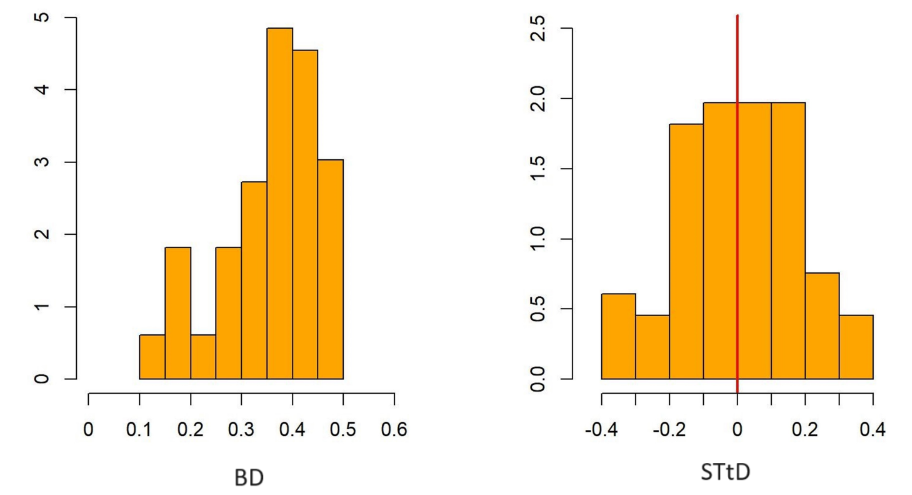
\includegraphics[width = 0.7 \textwidth]{Imagenes/comparacionBandas.png}
    \caption{Comparación visual de la medida banda de profundidad y la medida transformación de translación con signo de profundidad.}
    \label{fig:ComparaBandas}
\end{figure}

En contraste, en el histograma derecho se presentan las medidas utilizando la profundidad de banda transformada. Debido a la forma en que fue construida, se puede observar cierta simetría; además, se pueden identificar fácilmente los valores atípicos tanto por encima como por debajo de la curva.

%%%%%%%%%%%%%%%%%%%%%%%%%%%%%%%%%%%%%%%%%%%%%%%%%%%%%%%%%%
%%%%%%%% M E J O R A C I O N  D E  L A  T B D %%%%%%%%%%%%
%%%%%%%%%%%%%%%%%%%%%%%%%%%%%%%%%%%%%%%%%%%%%%%%%%%%%%%%%%

\section{Transformación de Variables Funcionales}

Como se detallará más exhaustivamente en el Capítulo \ref{Resultados}, una parte de la base de datos que se empleará para crear el modelo, consiste en mediciones de glucosa e insulina tomadas durante la prueba de tolerancia a la glucosa oral en los minutos $0$, $30$, $60$, $90$ y $120$. Estas observaciones se pueden considerar como curvas y, por lo tanto, constituyen los datos funcionales con los que se hará inferencia para proporcionar la probabilidad de padecer diabetes. 

Llámese $g(t)$ y $\eta(t)$ a las variables funcionales que representan los niveles de glucosa e insulina, respectivamente, donde $t = 0, 30, 60, 90, 120$. En la Figura \ref{fig:pairsTBD}, se muestran gráficos de dispersión, en los que el eje $x$ representa la profundidad de banda transformada con signo de la variable funcional glucosa, mientras que en el eje $y$ se muestra la profundidad de la variable funcional de insulina. Asi, cada punto representa la $STtD$ asociadas las curvas de glucosa e insulina de un individuo en la muestra. Según ciertos criterios determinados por mediciones de la OGTT (los cuales se detallarán en el Capítulo \ref{Resultados}), es posible realizar un prediagnóstico de los individuos clasificados como normales, prediabéticos y diabéticos. Estas categorías están coloreadas en los gráficos de dispersión, junto con la distribución de las bandas de profundidad transformada con signo en insulina y glucosa.

Un aspecto importante a destacar, en la Figura \ref{fig:pairsTBD}, es que la transformación de la banda de profundidad con signo de la variable glucosa muestra una distribución característica para cada categoría del prediagnóstico. En cuanto a la variable correspondiente a la insulina, no parece haber una separación clara entre las categorías. Sin embargo, en los gráficos de dispersión se puede observar con mayor claridad el comportamiento que se busca analizar.

\begin{figure}[H]
    \centering
    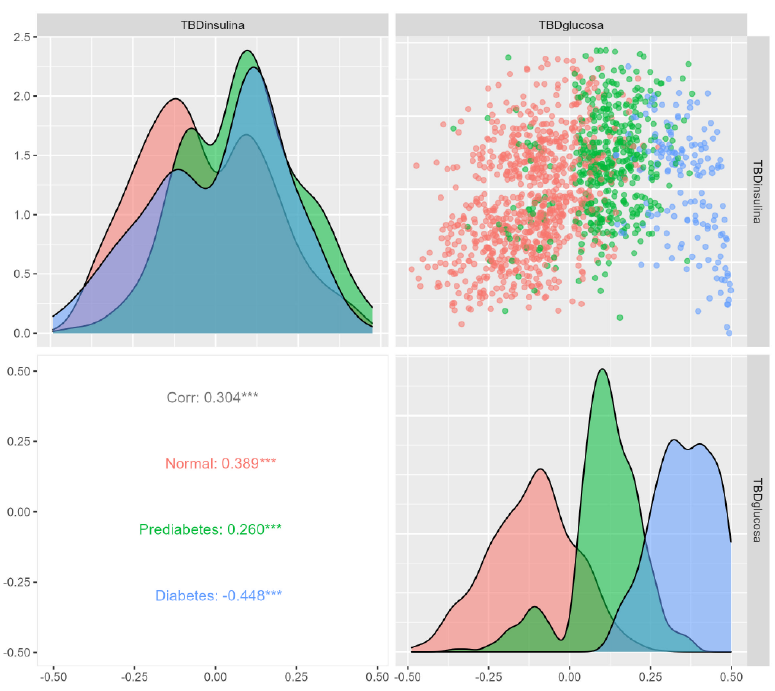
\includegraphics[width = 0.7 \textwidth]{Imagenes/pairsTBDS.png}
    \caption{Histogramas y gráficos de dispersión para las STtD's de las variables glucosa e insulina.}
    \label{fig:pairsTBD}
\end{figure}


Los altos niveles de glucosa se corresponden con bajos niveles de insulina, ya que la producción de insulina disminuye; lo cual se respalda con el signo negativo de la correlación en la categoría diabética. Esto es un poco complicado de ver en la Figura \ref{fig:pairsTBD} pero la correlación aclara esto. Por otro lado, los bajos niveles de glucosa también se asocian con bajos o medianos niveles de insulina, lo que indica un funcionamiento adecuado de la insulina en la categoría normal, donde el signo de la correlación es positivo.

En cuanto a los individuos prediabéticos se observa que presentan niveles altos tanto de glucosa como de insulina. Aunque la correlación es positiva, es importante notar que los valores de insulina alcanzan un máximo y luego descienden, lo que indica una posible falla irreversible de las células beta.

Además, en el punto $(0, 0)$, que corresponde a las medianas de cada variable, se puede observar una división por cuadrantes. Esto sugiere que, según esta división, se pueden clasificar a los individuos, y este será un punto de partida esencial para el presente trabajo. Sin embargo, es importante tener en cuenta que este punto puede ser modificado según criterios médicos, ya que podría ser preferible ajustarlo para disminuir la probabilidad de cometer errores de tipo $2$.

%%%%%%%%%%%%%%%%%%%%%%%%%%%%%%%%%%%%%%%%%%%%%%%%%%%%%%%%%
\subsection{Creación de Variable Respuesta}

Defínase el punto $\widetilde{TBD} = (\widetilde{TBD^g}, \widetilde{TBD^{\eta}})$ que representa los valores límite aceptables de glucosa e insulina para pacientes completamente sanos. A partir del punto $(\widetilde{TBD^g},\widetilde{TBD^{\eta}})$ se define la función cuadrante para cada observación como:

\begin{equation}
     C_ i = \left\{\begin{matrix}
1, & TBD_{i}^{g} < \widetilde{TBD^{g}}, TBD_{i}^{\eta} < \widetilde{TBD^{\eta}}\\
2, & TBD_{i}^{g} < \widetilde{TBD^{g}}, TBD_{i}^{\eta} > \widetilde{TBD^{\eta}}\\
3, & TBD_{i}^{g} > \widetilde{TBD^{g}}, TBD_{i}^{\eta} < \widetilde{TBD^{\eta}}\\
4, & TBD_{i}^{g} > \widetilde{TBD^{g}}, TBD_{i}^{\eta} > \widetilde{TBD^{\eta}}
\end{matrix}\right.
\end{equation}

\begin{enumerate}
    \item El primer cuadrante, denotado como $C_i = 1$, corresponde al cuadrante inferior izquierdo y se asocia con los pacientes \textbf{completamente sanos}. Estos pacientes presentan niveles estables tanto de glucosa como de insulina.
    \item El segundo cuadrante, asociado con $C_i = 2$, comprende a los pacientes que presentan \textbf{resistencia a la insulina o predisfunción de las células beta}. Estos pacientes han comenzado a aumentar sus niveles de insulina para mantener estable su glucosa. Quienes están en este cuadrante tienen una alta probabilidad de regresar al cuadrante $1$ mediante la mejora de hábitos dietéticos y de ejercicio físico.
    \item El tercer cuadrante, relacionado con $C_i = 3$, se refiere a los pacientes con \textbf{resistencia a la insulina o estrés en las células beta}. Estos pacientes, a pesar de experimentar un aumento en sus niveles de insulina, no logran mantener estables sus niveles de glucosa; lo cual indica una disminución en su sensibilidad a la insulina. Tienen una probabilidad muy baja de regresar a los cuadrantes 1 o 2 mediante la mejora de hábitos dietéticos y de ejercicio, lo que sugiere que es probable que hayan desarrollado resistencia a la insulina.
    \item En el cuarto cuadrante, identificado como $C_i = 4$, se encuentran los pacientes con \textbf{resistencia a la insulina y disfunción evidente de las células beta}. Estos pacientes requieren la administración de insulina para mantener estables sus niveles de glucosa, y tienen escasas posibilidades de regresar a alguno de los cuadrantes previos.
\end{enumerate}

Usando los cuadrantes se define la siguiente función

\begin{equation}
    m_i= \begin{cases}
    \widehat{F}^g\left(T B D_i^g\right) \cdot \widehat{F}^\eta\left(T B D_i^\eta\right), & C_i=1, \\ \widehat{F}^g\left(T B D_i^g\right) \cdot\left(1-\widehat{F}^\eta\left(T B D_i^\eta\right)\right), & C_i=2, \\ \left(1-\widehat{F}^g\left(T B D_i^g\right)\right) \cdot\left(1-\widehat{F}^\eta\left(T B D_i^\eta\right)\right), & C_i=3, \\ \left(1-\widehat{F}^g\left(T B D_i^g\right)\right) \cdot \widehat{F}^\eta\left(T B D_i^\eta\right), & C_i=4,\end{cases}
\end{equation}


donde $\widehat{F}^g$ y $\widehat{F}^{\eta}$ representan la función empírica de los valores de \textit{Signed Translation transformed Depth} de los datos funcionales correspondientes a la glucosa y la insulina, respectivamente. Esta función desempeña el papel de funciones de ponderación. Posteriormente se procede a computar la siguiente función:

\begin{equation}
    F B I / G C_i= \begin{cases}\left(M_1-m_i\right) / M_1, & C_i=1, \\ \left(m_i-M_2\right) / M_2, & C_i=2, \\ \left(m_i-M_3\right) / M_3-1, & C_i=3, \\ \left(m_i-M_4\right) / M_4-2, & C_i=4,\end{cases}
\end{equation}

donde $M_k =  \displaystyle \max_{m_i \in C_k} m_i$ para $k = 1, 2, 3, 4$ y $FBI/GC$ son las siglas de \textit{Functional Based Insulin/Glucose Classification}.


Con el fin de establecer un cierto orden en la condición de las células beta, se realiza un escalado utilizando el máximo de cada cuadrante y restando una constante. Este procedimiento permite estandarizar los valores y facilitar la comparación entre diferentes grupos de pacientes proporcionando una medida relativa de la función de las células beta en relación con el estado de salud.

\begin{enumerate}
    \item En el cuadrante $1$, asociado con pacientes \textbf{completamente sanos}, la variable respuesta se encuentra en el rango $0 \leq \text{FBI/GC} \leq 1$.
    \item En el cuadrante $2$, correspondiente a los pacientes con \textbf{resistencia a la insulina o predisfunción de la célula beta}, la variable creada anteriormente se encuentra en el rango $-1 \leq \text{FBI/GC} \leq 0$.
    \item En el cuadrante $3$, que comprende a los pacientes con \textbf{resistencia a la insulina y estrés en la célula beta}, se tiene que $-2 \leq \text{FBI/GC} \leq -1$.
    \item En el cuadrante 4 se encuentran los pacientes con \textbf{resistencia a la insulina y disfunción evidente de la célula beta}, donde $-3 \leq \text{FBI/GC} \leq -2$.
\end{enumerate}

 Luego de llevar a cabo todos los cálculos mencionados anteriormente, se ha logrado construir una variable numérica que encapsula toda la información esencial extraída de los datos funcionales obtenidos de las curvas de glucosa e insulina. Esta variable condensa de manera efectiva la complejidad de los datos originales en una forma que resulta conveniente para el ajuste del modelo de regresión cuantil.